% !TEX root = ../Masters.tex
\chapter{Evaluation of DGEL}
DGEL consists of to main modules: \textit{generation} and \textit{evaluation}.
The evaluation module consists of the fitness component which evaluates who good the L-system plants are.
The remaining components are part of the generation component which generates plants, and uses the evaluation module to generate \textit{good} plants.
To answer if DGEL solves the research questions, both modules have to be evaluated.
The generation module will be evaluated in a technical manner to determine if it performs well or not.
The evaluation module will be evaluated using humans as to answer if the fitness function properly rates plants as aesthetically pleasing or not.

\section{Evaluation of the Generation Module}
\subsection{Method}
As explained in Section~\ref{sec:overview} and shown in Figure~\ref{fig:dgel}, there are two main processes involved in generating the model for the L-system plants: \textit{SA} and \textit{GE}.
The remaining steps are dependent on the model and do not create variations on the same model.
Thus GE and SA are the two processes of interests to evaluate.

% GE SA vs GE uniform - need data, how to measure?

\subsubsection{Grammar Evolution Parameters}
GE, as with GA, depends on multiple parameters, and with tournament sampling there are even more.
Thus, before evaluation the GE process, good parameters should be found.
Additionally, seeing what parameters are needed for a good performing GE may reveal additional properties of it.
The parameters were found using a combined manual and automated approach by searching the parameter space in multiple steps.
The idea was not to find the optimal parameters, but rather to find some parameters that made the GE produce an individual with good fitness within a reasonable time.
It was assumed that the size parameters --- population size and number of generations --- are the baseline parameters for GE and thus should be found first.
Then the tournament size for the tournament selection strategy should be found.
Then good parameters for the recombination rates --- crossover rate and mutation rate --- should be found.
Finally the parameter for the GE gene duplication operator should be found.
% Reason for these assumptions?

To search for the GE parameters, a breadth-first graph search inspired approach was used.
An example is shown in Figure~\ref{fig:parameter-search}.
The approach tests a combination of parameters by doing 20 GE runs with those parameters and using the mean fitness score of the best individual from each run.
If the score is an improvement of the previous score, the node will be considered an improvement and it will consider the neighboring nodes in the graph by increasing the parameter values.
Otherwise, the current parameter values will be considered as not improving the performance and thus be discarded.
When there are no more improvements, the parameter values that produced the best score will be returned.
The parameter values will start at a small value and increase in an exponential fashion.
This is based on the assumption that the parameters are more sensitive when the values are small.
All of the parameter searches, except for the reproduction parameter search, will increase with a multiplicative of 2.
Because the reproduction rate parameters are bounded ($[0, 1]$) and to cover the whole range with a reasonable amount of steps, custom steps of 0.01, 0.1, 0.5 and 1 are used.

\begin{figure}
    \centering
    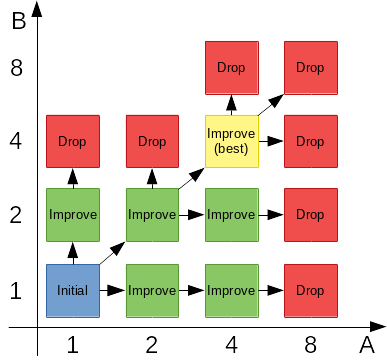
\includegraphics[width=0.6\textwidth]{figures/parameter-search}
    \caption{Example of a GE parameter search}
    \label{fig:parameter-search}
\end{figure}

\subsubsection{Grammar Evolution Test}
The reason for using GE is to search the space in an efficient way.
To see if it is doing this, it needs to be compared to a brute-force approach that finds completely random samples in the space and picks the best of them.
Thus, the hypothesis is that DGEL GE finds plants with better fitness scores than brute-force does (\textbf{H1}).

To make a fair comparison, the brute-force should generate as many individuals as the GE generates and modifies (through mutation or crossover)
This way, both methods will ``generate'' the same amount of individuals, either being completely new individuals or modifications of existing individuals.
GE uses a fixed number of generations and population size, resulting into a fixed number of total individuals: $individuals = population + population * generations$.
Thus the brute-force method will generate $individuals$ individuals.

Because both methods depend on a random seed, an average of multiple runs will have to be used.
A sample size of 11 was selected as balanced choice between sample size and duration.

\subsubsection{Simulated Annealing}
% \begin{itemize}
% 	\item Can SA and the grammar distribution be used to find portions of the parameter space that generate better L-system plants?
% 	\item Does SA enable GE to find better L-system plants?
% 	\item Can SA find multiple portions of the parameter space that each generate unique-looking plants?
% \end{itemize}
The main purpose of using SA with a grammar distribution is to improve the efficiency of the remaining components of DGEL by focusing the search space on a good area.
Based on this a hypothesis can be formulated: An SA-optiomized grammar distribution can find better individuals than a uniform grammar distribution (\textbf{H2}).
An important word in the hypothesis is \textit{can}, because this means that the hypothesis does not imply that \textit{all} SA-optimized grammar distributions will find better individuals.

SA is used as described in previous sections to find an optimized grammar distribution, and the progress of it is plotted to see if it makes any meaningful progress.
Then, to test the hypothesis a comparison is made between the average fitness of L-systems randomly generated by a uniform grammar distribution and L-systems randomly generated by an SA-optimized grammar distribution.
The L-systems are generated in a brute-force manner, not using any evolutionary approach such as GE.

If \textbf{H2} is supported, we can further hypothesize that \textit{GE} with an SA-optimized grammar distribution can find better individuals than with a uniform grammar distribution (\textbf{H3}).
% Have run tests with 160800 individuals, but GE with uniform is already so good that it isn't comparable.
% Thus we need a better comparison (fewer individuals? Time to convergence?)
%To test this hypothesis, the performance of GE with a uniform grammar distribution is compared to the performance of GE with an SA-optimized grammar distribution.
%Both GE processes were run 11 times, each time extracting the best L-system, before taking the mean of the best L-systems and using a t-test to test if the means were different.

% Finally,check variation of SA. How to? Right now I can only manually check some examples.

\subsection{Results}
\subsubsection{Grammar Evolution Parameters}
Figure~\ref{fig:size-sampling} shows the search of the population size and number of generations to be used for the GE process.
The search was prematurely stopped because at around either 1600 number of generations or population size the duration became unreasonable long.
As seen, a minimum of either a population size of 200 or 200 generations is required for a reasonable performance.
Additionally, for any number of generations, a population size of 200 makes a notable improvement.
From this point on, there is a steady improvement from scores around 0.8 to 0.9 with both parameters increasing towards 1600.
% Actually draw this line?
Outside a line drawn through 800, 400 and 400, 800 there does not seem to be any notable improvement, while the duration increases by a large amount.
The parameter values that yielded the best fitness was $generations = 200$ and $population size = 800$, and they did it within a reasonable duration.
The duration of it is significantly smaller than other parameter values that yield approximately the same fitness.
Thus, these parameter values were selected for use.

\begin{figure}
    \centering
    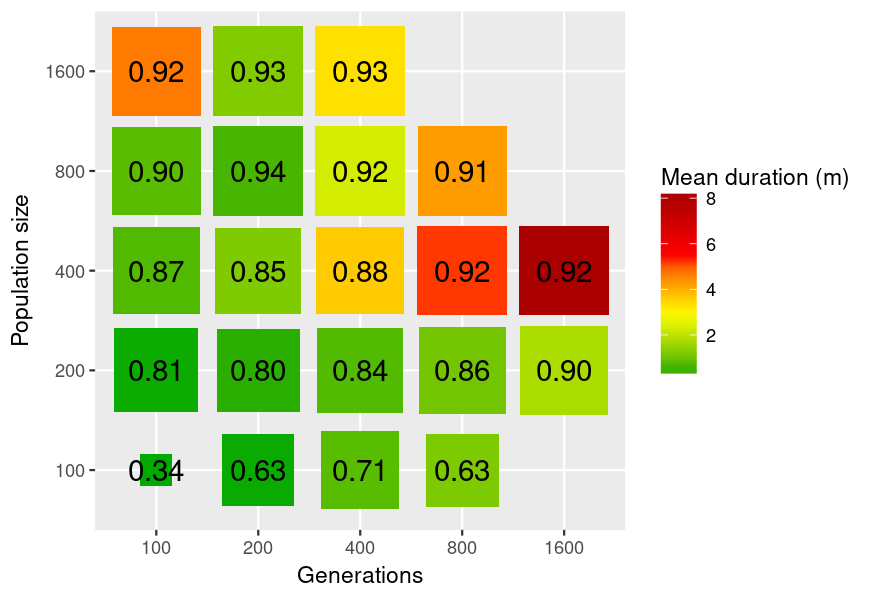
\includegraphics[width=0.8\textwidth]{figures/ge-size-sampling}
    \caption[Visualized search of GE population size and number of generations]{Visualized search of GE population size and number of generations. Numbers are the mean of best fitness scores, box sizes are a representation of that number, and colors represent the mean duration of the GE.}
    \label{fig:size-sampling}
\end{figure}

Figure~\ref{fig:tournament-sampling} shows the search of the tournament size.
Contrasted to the other searches, this is a one-dimensional search.
% Possibly do a significance test. Need to re-run to generate raw data...
As seen in the figure, the search did not find any improvements at all.
Thus the tournament size was kept at the lowest value, i.e.\ 2.

\begin{figure}
    \centering
    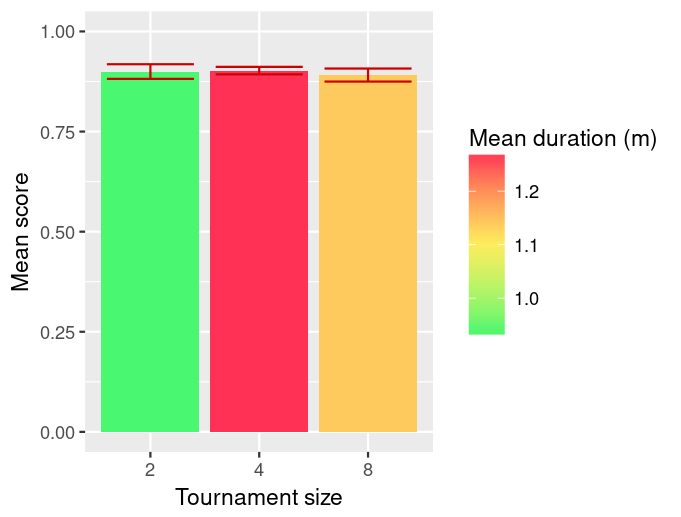
\includegraphics[width=0.7\textwidth]{figures/ge-tournament-sampling}
    \caption[Visualized search of the GE tournament selection tournament size]{Visualized search of the GE tournament selection tournament size with standard error}
    \label{fig:tournament-sampling}
\end{figure}

Figure~\ref{fig:recombination-sampling} shows the search of the recombination parameters: mutation rate and crossover rate.
There is a general improvement in fitness with both increasing mutation rate and crossover rate until the crossover rate reaches 1 where it suddenly turns for the worse.
Thus the crossover rate should at least be below 1.
Additionally, the crossover rate seems to be the parameter that contributes less to an improved fitness and increases the duration the most.
Thus the mutation rate should be the most important parameter.
The best fitness score is provided by a mutation rate of 1 and crossover rate of 0.5, further indicating this.

% Also did an ANOVA on this, could mention.
Figure~\ref{fig:recombination-sampling-variance} shows the standard deviations in the same search.
The pattern is similar to that of the mean fitness scores.
The most stable performance is provided by a mutation rate of 1 and crossover rate of 0.5.
Thus the recombination parameters will be using these values.

\begin{figure}
    \centering
    \begin{subfigure}{0.57\textwidth}
        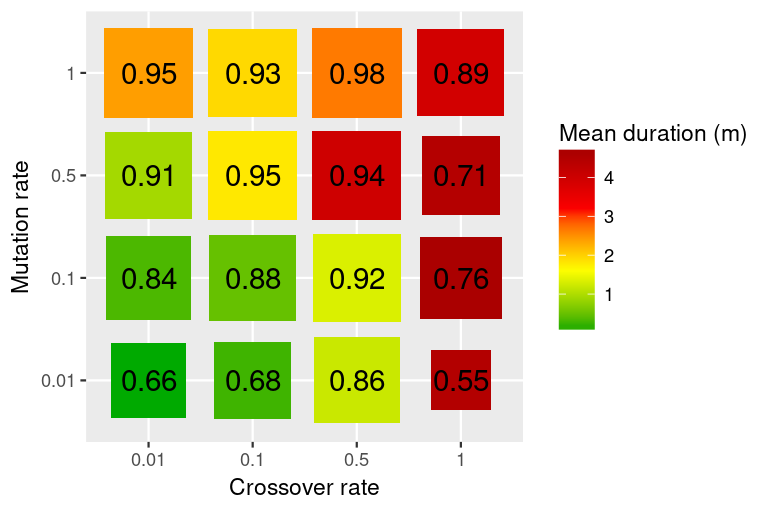
\includegraphics[width=\textwidth]{figures/ge-recombination-sampling}
        \caption{Mean of best fitness scores as numbers and sizes, with duration as colors}
        \label{fig:recombination-sampling}
    \end{subfigure}
    ~
    \begin{subfigure}{0.4\textwidth}
        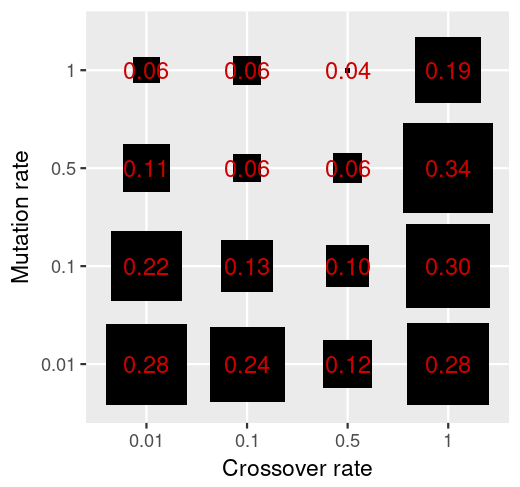
\includegraphics[width=\textwidth]{figures/ge-recombination-sampling-variance}
        \caption{Standard deviation}
        \label{fig:recombination-sampling-variance}
    \end{subfigure}
    \caption{Visualized search of the GE recombination parameters}
\end{figure}

% WHAT ABOUT DUPLICATION RATE
All of the GE parameters are summarized in Table~\ref{tab:ge-parameters}.

\begin{table}
    \centering
    \begin{tabular}{| l | l |}
    \hline
    \textbf{Parameter} & \textbf{Value} \\ \hline
    Population size & 800 \\
    \hline
    Generations & 200 \\
    \hline
    Tournament size & 2 \\
    \hline
    Mutation rate & 1.0 \\
    \hline
    Crossover rate & 0.5 \\
    \hline
    Duplication rate & 0 \\
    \hline
    \end{tabular}
    \caption{GE parameter values selected based on searches}
    \label{tab:ge-parameters}
\end{table}

\subsubsection{Grammar Evolution Test}
\begin{figure}
    \centering
    \begin{subfigure}{0.4\textwidth}
        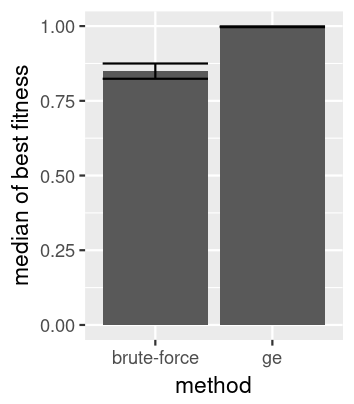
\includegraphics[width=\textwidth]{figures/ge-random}
        \caption{Median of best fitness with MAD}
        \label{fig:ge-random}
    \end{subfigure}
    ~
    \begin{subfigure}{0.4\textwidth}
        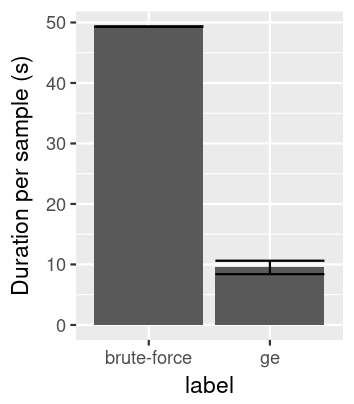
\includegraphics[width=\textwidth]{figures/ge-random-duration}
        \caption{Mean duration with SE}
        \label{fig:ge-random-duration}
    \end{subfigure}
    \caption{GE and random performance compared}
\end{figure}

Figure~\ref{fig:ge-random} shows the comparison of GE against random samples.
A Shapiro-Wilk normality test suggests that the brute-force sample distribution can be assumed to be normally distributed (p >= 0.05, W = 0.97), while the GE sample distribution can not (p < 0.05, W = 0.46).
A robust Brown-Forsythe Levene-type test suggests that the variances of the distributions can be considered equal (p >= 0.05, statistic = 0.09).
Because there are non-normal distributions and different variances, the Mann-Whitney U test will be used.
GE has a median score of 1.00, while random has 0.85 (difference of 0.15).
The Mann–Whitney U test suggests that the true location shift of the distributions is greater than 0 (p < 0.05, U = 117).
% Could run test on this as well, but necessary??

% Caused by tournament sampling.
Additionally, Figure~\ref{fig:ge-random-duration} shows the mean duration of the methods where GE is about 5 times faster than random.
A Shapiro-Wilk normality test suggests that both the brute-force and GE samples can be assumed to be normally distributed (p >= 0.05, W = 0.89 and p >= 0.05, W = 0.93 respectively).
A robust Brown-Forsythe Levene-type test suggests that the variances of the distributions can be considered unequal (p < 0.05, statistic = 17.13).
Because the distributions can be assumed to be normally distributed and the variances can be assumed to be unequal, the Welch's t-test will be used.
GE has a mean duration of 9.51, while random has 49.33 (difference of -39.82).
The Welch's two-sample t-test suggests that the true difference in means are not 0 (p < 0.05, t = -35.90, df = 10.02)

\subsubsection{Simulated Annealing}
\begin{figure}
    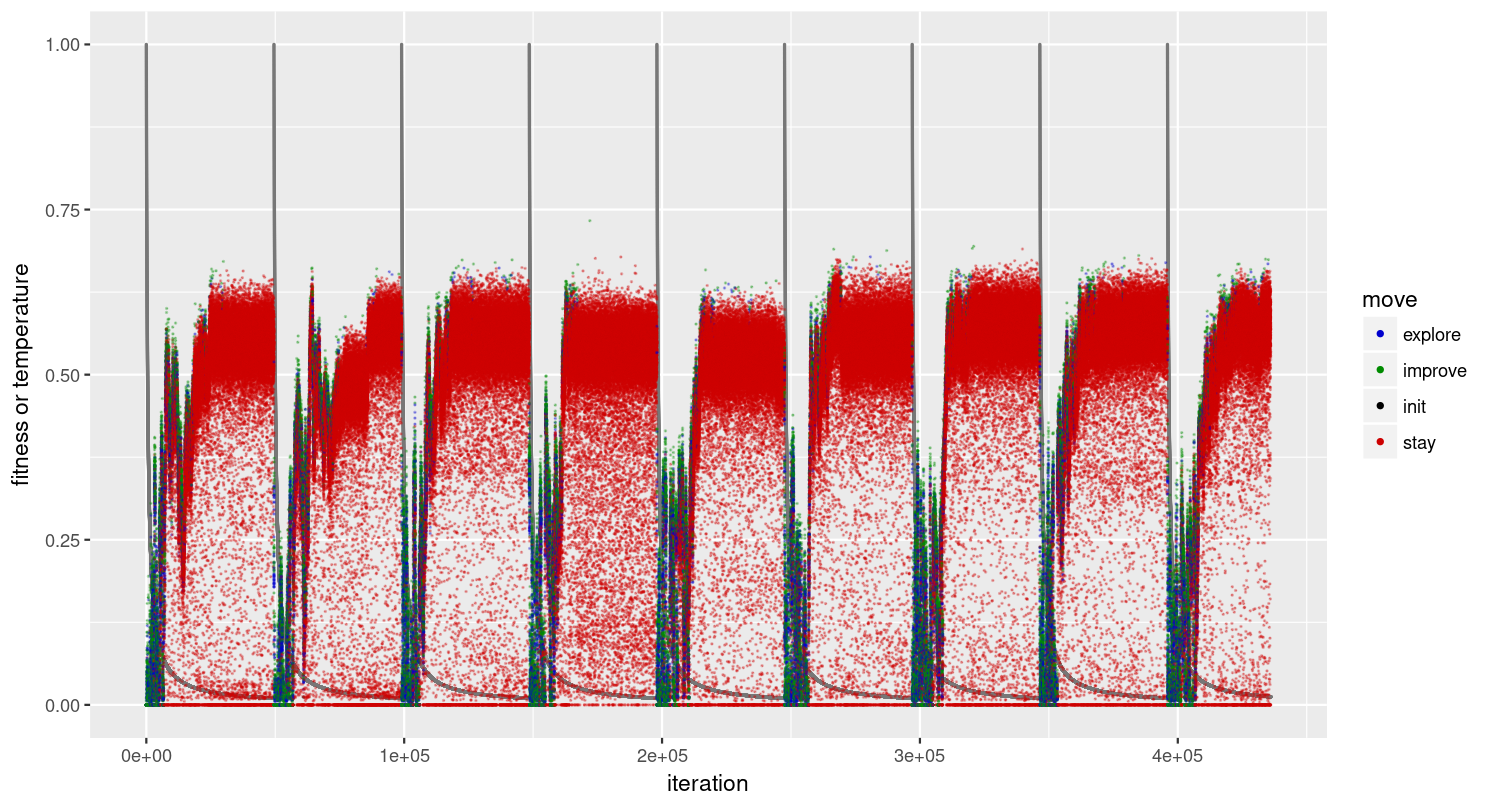
\includegraphics[width=\textwidth]{figures/sa-progress}
    \caption{The complete SA process with multiple re-annealings}
    \label{fig:sa-progress}
\end{figure}

Figure~\ref{fig:sa-progress} shows the progress of one SA run, and Figure~\ref{fig:sa-progress-close} shows a close-up of the first annealing.
The run had a maximum of 2000 moves per dimension and a cooldown rate of 0.002.
The grammar distribution evaluation had a minimum 32 samples and an error threshold of 0.004.
In total this resulted into 436000 moves over 9 annealings.
As seen in the figure, for each annealing there is a general improvement from a fitness score of 0 to around 0.6.
The SA process explores the space in the beginning, moving both up and down in score, and then gradually focuses more on hill climbing towards the end.
Each annealing generally reach a plateau before being halfway through the annealing process, from when nearly all mutations are worse and thus it chooses to stay, though the second annealing is slower to reach the plateau.
The fourth annealing found one exceptionally good grammar distribution with a score of almost 0.75, but when the same grammar distribution was measured over 100000 samples its score was 0.61 (SD = 0.25).
Thus the score measured in the SA process may have been inaccurate.
As this distribution was the one with the best score during the SA process, it will be the one used for further analysis.

\begin{figure}
    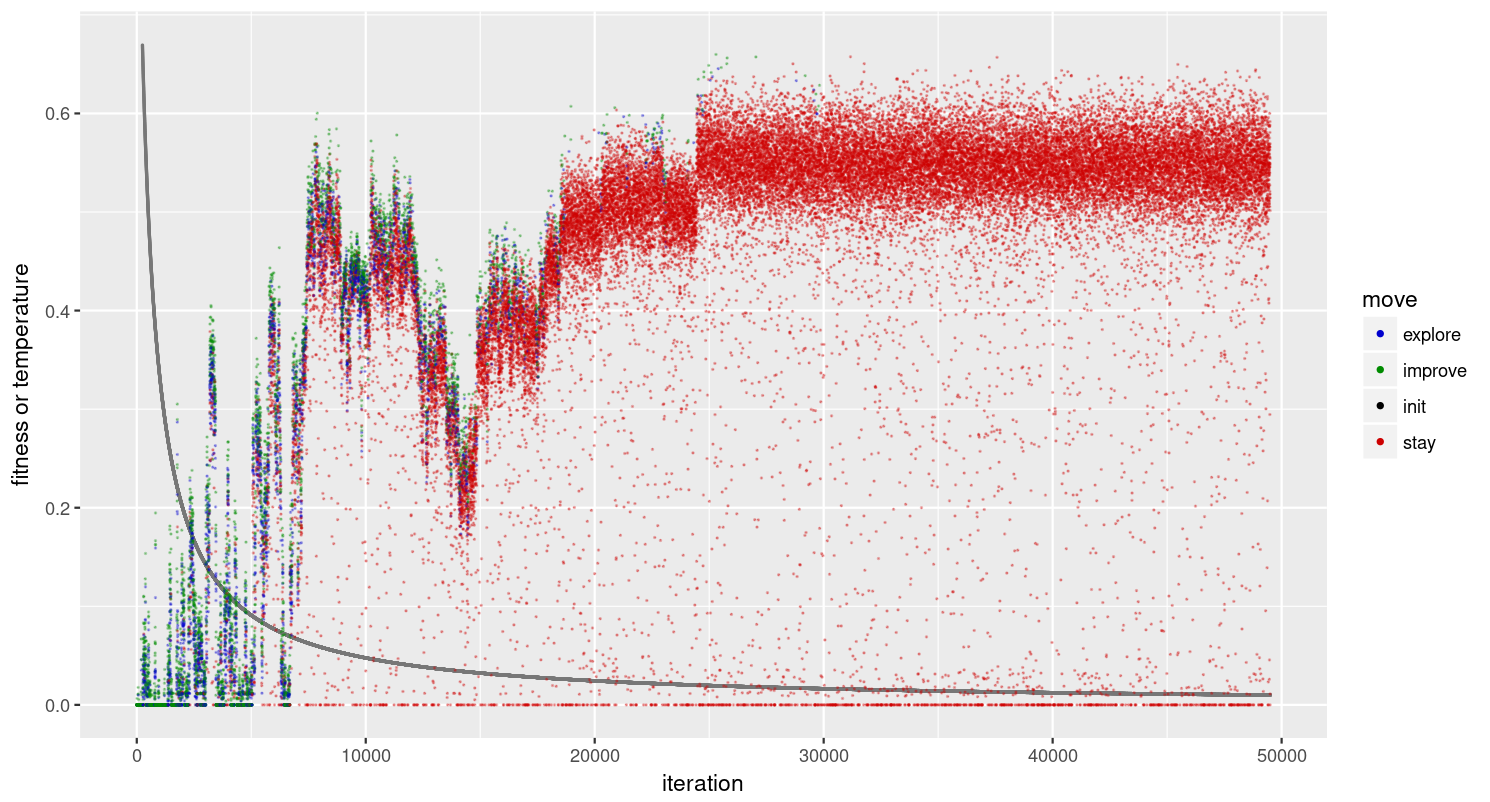
\includegraphics[width=\textwidth]{figures/sa-progress-close}
    \caption{Close-up of the first annealing of the SA process}
    \label{fig:sa-progress-close}
\end{figure}

Seen in Figure~\ref{fig:sa-progress-close} the points cluster around the same score.
At the same time there are some points spread fairly uniformly between the clustering and 0.
Additionally there is a clustering at exactly 0.

\begin{figure}
    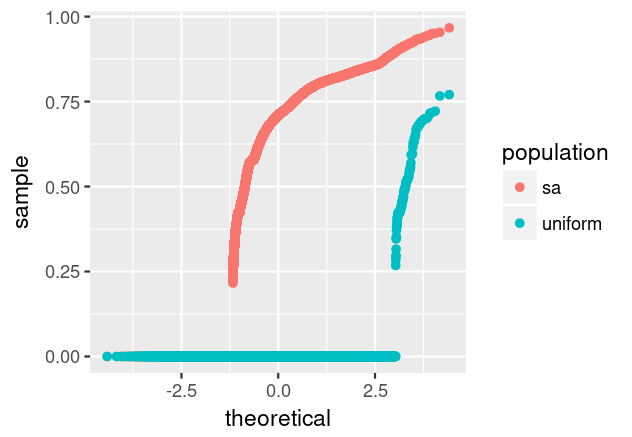
\includegraphics[width=\textwidth]{figures/sa-qq}
    \caption{Q-Q plot of SA and uniform sample populations}
    \label{fig:sa-qq}
\end{figure}

As the sample size (n = 100000) is too large for a Shapiro-Wilk normality test, a Q-Q plot is used.
It can be seen in Figure~\ref{fig:sa-qq}, and it is clear that the distributions are not normally distributed.
Even with all 0 scores removed, the data does not appear normally distributed.
A robust Brown-Forsythe Levene-type test shows that the variances of the distributions can not be considered equal (p < 0.05).

\begin{figure}
    \centering
    \begin{subfigure}{0.48\textwidth}
        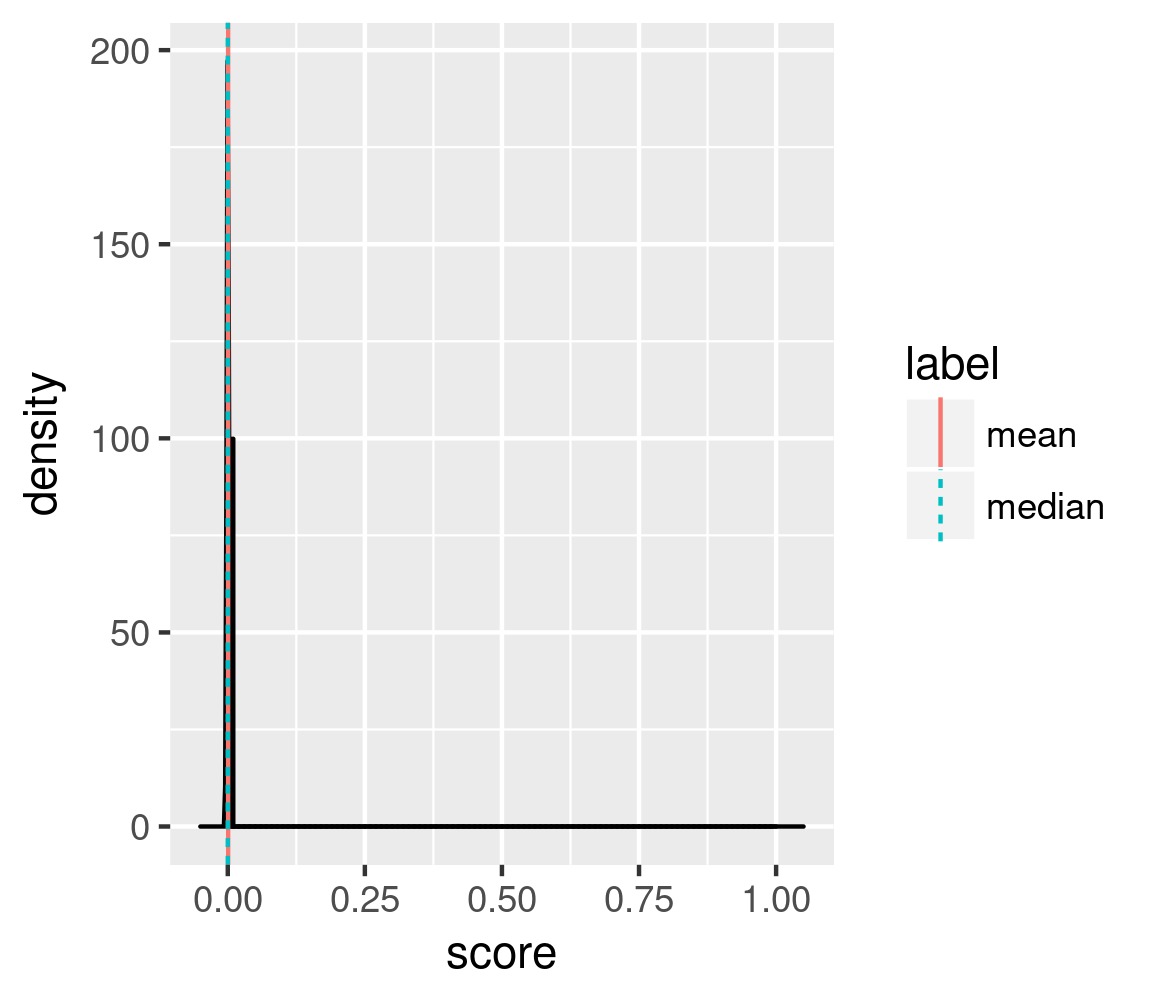
\includegraphics[width=\textwidth]{figures/uniform-population}
        \caption{Complete sample population}
        \label{fig:uniform-population}
    \end{subfigure}
    ~
    \begin{subfigure}{0.48\textwidth}
        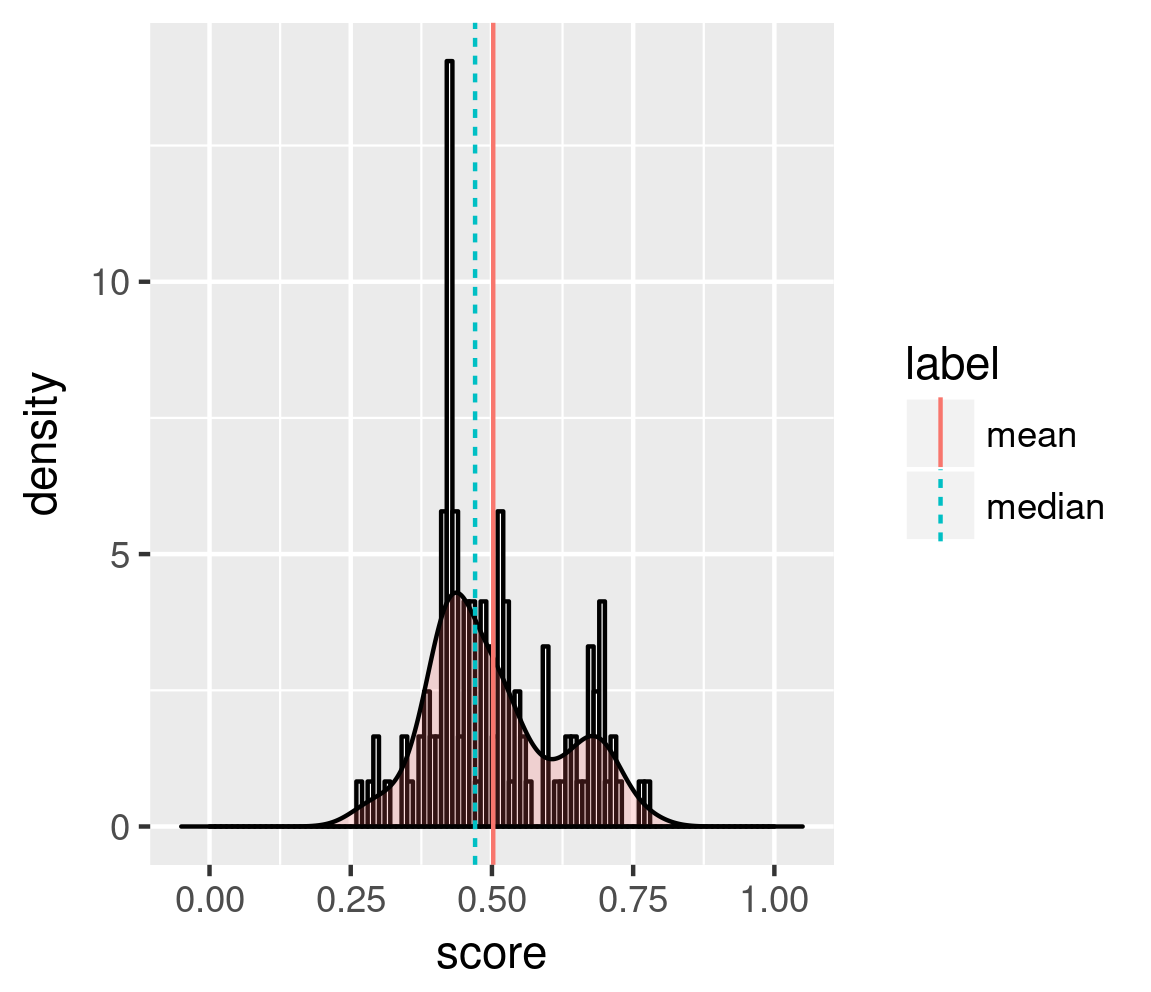
\includegraphics[width=\textwidth]{figures/uniform-population-no0}
        \caption{Sample population without samples with score 0}
        \label{fig:uniform-population-no0}
    \end{subfigure}
    \caption{Sample population of L-systems generated using a uniform grammar distribution}
\end{figure}

\begin{figure}
    \centering
    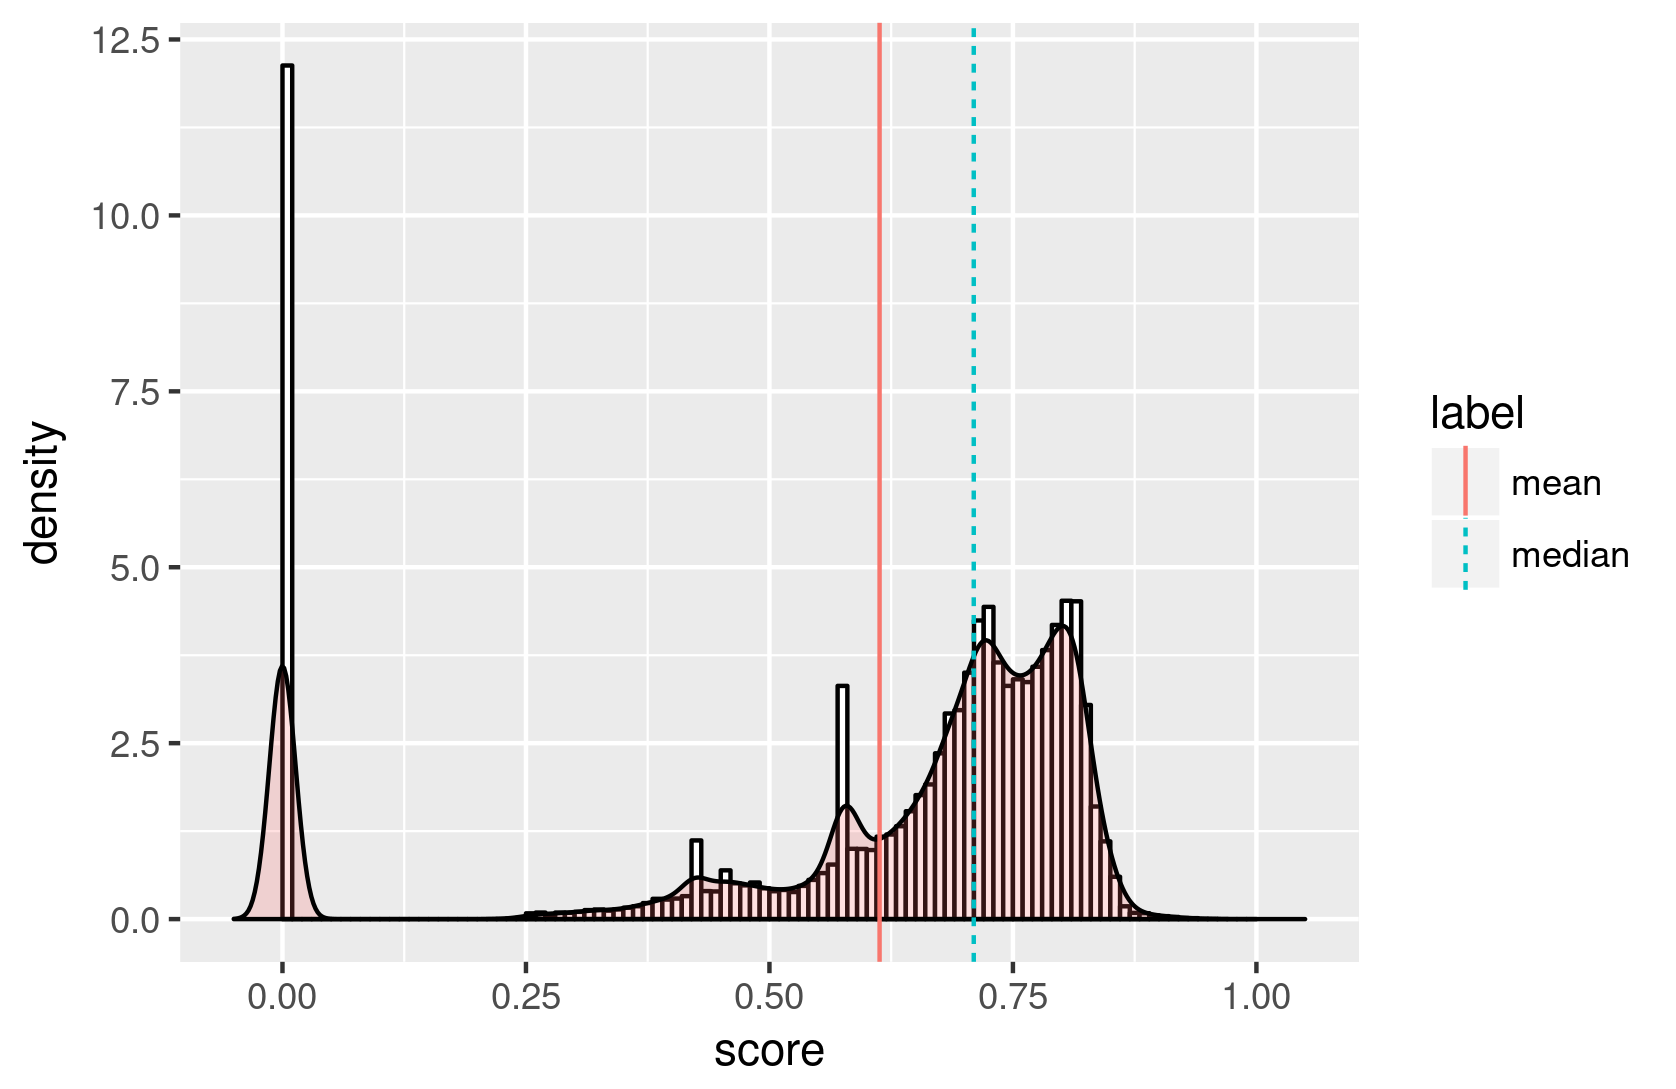
\includegraphics[width=0.8\textwidth]{figures/sa-population}
    \caption{Sample population of L-systems generated using the SA-optimized grammar distribution}
    \label{fig:sa-population}
\end{figure}

Figure~\ref{fig:uniform-population} shows the uniform grammar distribution' sample distribution, where practically the whole population has a score of 0.
When removing all zero-scored individuals, another distribution presents itself in Figure~\ref{fig:uniform-population-no0}.
Here, a somewhat double bell-shaped distribution around the score 0.5 with a high concentration at around 0.4 is revealed for the remaining 121 individuals (0.12\% of the total).
Figure~\ref{fig:sa-population} shows the SA grammar distribution's distribution of fineness scores.
87.87\% of the SA sample population have a score larger than 0, compared to 0.121\% in the uniform sample population.
%Thus the SA grammar distribution helps avoid most of the worst L-systems.
%As the distribution is skewed to the left, the median may be a better estimate of the population average.

\begin{figure}
    \centering
    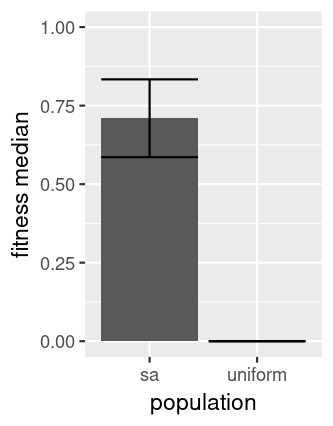
\includegraphics[width=0.4\textwidth]{figures/sa-uniform}
    \caption{Random population with uniform grammar distribution compared to SA-optimized grammar distribution}
    \label{fig:sa-uniform}
\end{figure}

Figure~\ref{fig:sa-uniform} shows a comparison of L-system populations generated by the grammar distribution found by SA in Figure~\ref{fig:sa-progress} and a uniform grammar distribution.
The SA grammar distribution has a median of 0.71 (MAD: 0.12), compared to 0.00 (MAD: 0.00) for the uniform grammar distribution.
A Mann–Whitney U test on the full sample suggests that the true location shift is not zero (p < 0.05, U = 608550000).
Even with all individuals with score 0 removed, the SA grammar distribution's median score is higher with a median of 0.72 (MAD: 0.10) compared to 0.47 (MAD: 0.08), though the difference of 0.25 is smaller.
A Mann–Whitney U test on the sample without zero scores still suggests that the true location shift is not zero (p < 0.05, U = 1318100).

% might split these into separate figures and put them inbetween the above paragraphs
\begin{figure}
    \centering
    \begin{subfigure}{0.48\textwidth}
        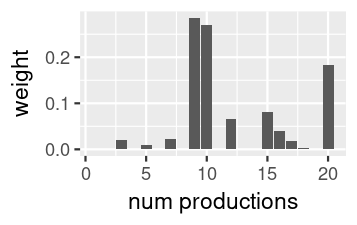
\includegraphics[width=\textwidth]{figures/sa-dist-prod}
        \caption{1*20production}
        \label{fig:sa-dist-prod}
    \end{subfigure}
    ~
    \begin{subfigure}{0.48\textwidth}
        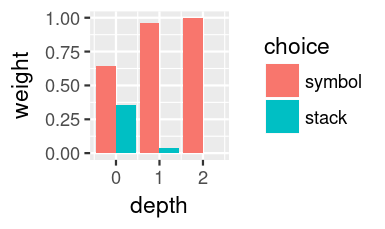
\includegraphics[width=\textwidth]{figures/sa-dist-stack}
        \caption{symbol / stack}
        \label{fig:sa-dist-stack}
    \end{subfigure}
    \\
    \begin{subfigure}{0.98\textwidth}
        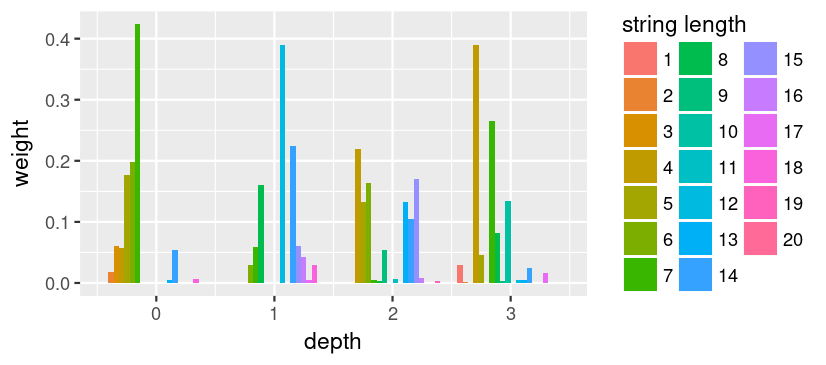
\includegraphics[width=\textwidth]{figures/sa-dist-strlen}
        \caption{1*20(symbol / stack)}
        \label{fig:sa-dist-strlen}
    \end{subfigure}
    \\
    \begin{subfigure}{0.4\textwidth}
        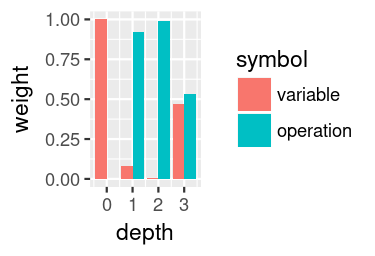
\includegraphics[width=\textwidth]{figures/sa-dist-sym}
        \caption{variable / operation}
        \label{fig:sa-dist-sym}
    \end{subfigure}
    ~
    \begin{subfigure}{0.57\textwidth}
        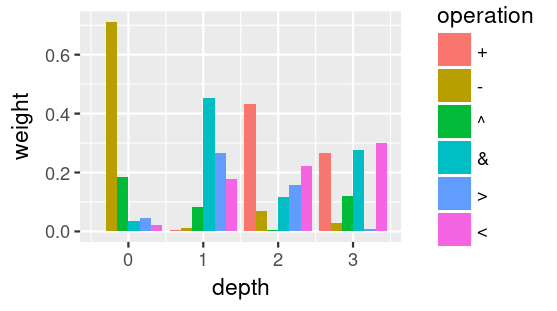
\includegraphics[width=\textwidth]{figures/sa-dist-op}
        \caption{"+" / "-" / "\textasciicircum" / "\&" / ">" / "<"}
        \label{fig:sa-dist-op}
    \end{subfigure}
\end{figure}
\begin{figure}
    \ContinuedFloat
    \begin{subfigure}{0.98\textwidth}
        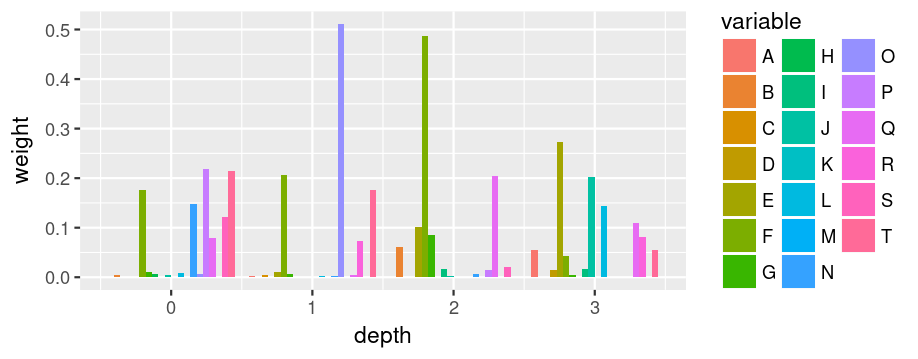
\includegraphics[width=\textwidth]{figures/sa-dist-var}
        \caption{\%x41-55}
        \label{fig:sa-dist-var}
    \end{subfigure}
    \caption[SA-optimized grammar distribution]{SA-optimized grammar distribution. Captions are the respective parts of Listing~\ref{lst:grammar}.}
    \label{fig:sa-dist}
\end{figure}

The grammar distribution found in the SA process is shown in Figure~\ref{fig:sa-dist}.
As seen in Figure~\ref{fig:sa-dist-prod}, this grammar distribution favors around 10 production rules in the L-system, though 20 productions is also a strong contender.
Figure~\ref{fig:sa-dist-stack} shows that it always favors symbols over stacks, starting at around 60\% symbols in the top depth, then around 90\% symbols in the next depth, and 100\% symbols in the final depth.
This makes all of the distributions at depth 3 irrelevant as they will never be used.
It favors shorter strings in depth 0, but not too short strings, as seen in Figure~\ref{fig:sa-dist-strlen}.
While in depth 1 and 2 it favors medium short and medium long strings.

Figure~\ref{fig:sa-dist-sym} shows that it only allows variables in depth 0, while its nearly the inverse in depth 1 and 2.
This is interesting as an operation has no effect if it is not followed by a variable.
Thus depth 2, along with depth 3, is not contributing anything to the plant, but depth 2 is still wasting instructions.
Depth 1 also has only about 10\% chance of a variable, meaning that most of the drawing will happen in depth 0, which in turn means less branching.

The operation distribution in Figure~\ref{fig:sa-dist-op} has a strong tendency of yawing to the right (\texttt{-}) than the left (\texttt{+}) in depth 0.
In depth 1 it barely allows yawing at all, while in depth 2 it is the opposite with a strong focus on \texttt{+}.
The other rotations (pitch and roll) also have one-sided tendencies, but not as strong.
Among all of the 20 variables available, \texttt{F} is the only variable that is an instruction, the draw line instruction.
Figure~\ref{fig:sa-dist-var} shows that it is included and is in fact one of the stronger variables in the distribution.
Only 3--4 of the variables have a strong weight in each of the depths.

\begin{figure}
    \centering
    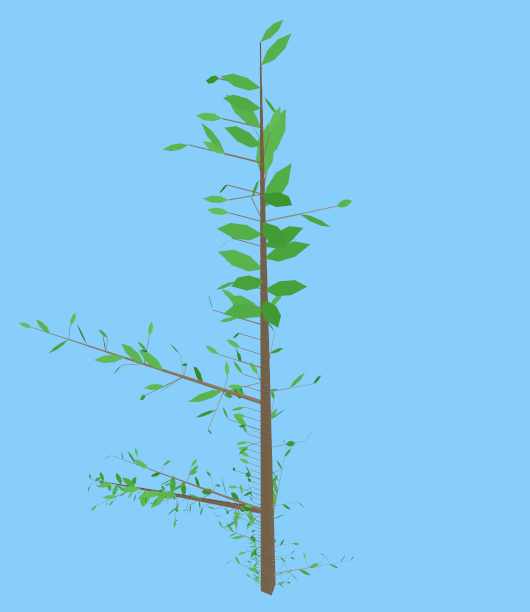
\includegraphics[width=0.6\textwidth]{figures/sa-plant}
    \caption[Example plant generated by the SA-optimized grammar distribution]{Example plant generated by the SA-optimized grammar distribution, fitness 0.78}
    \label{fig:sa-plant}
\end{figure}

\begin{lstlisting}[caption=L-system representation of plant in Figure~\ref{fig:sa-plant}, label=lst:sa-plant, float]
axiom: NT[>>&&&&>&&&F[++++<<]]P[<<&^[>-+<+>]&><&&&&&O]P
F -> Q[O&^&&&^&<>O[<<+++++^>++<++&][++++-]&>]NT[^>R>&>[<<&<+&+&<+&+-<]<<>&&]P
L -> [O&<<>&^&&&&>]S[^<[+++-<<>>++<<+<-]^>&<<&>&&>F^>]T[<<&><^&&O&<>]
N -> N[><&<^&<<&&^&&T][&>[+-<<>+++&+&<+][+++++&><++><<^-]&&&>]PN[&&>&>T&&&&^&><<&]
P -> [&&&O>&>&&>>&&F]F[<&&&&&&>&&&&]TF
S -> [><&<&&>&]TSQS[&T<<<>[>++-+]<<&&>]T
T -> PT[>&^>&&&>&&R&&<>>]
\end{lstlisting}

% Try to connect this to the above even more.
An example of a plant generated with the SA-optimized distribution can be seen in Figure~\ref{fig:sa-plant}, and its L-system is found in in Listing~\ref{lst:sa-plant}.
This plant is very tall and straight, has few branches and few fractal patterns.
The L-system goes to depth 2, but depth 2 never includes any symbols, thus not being relevant.
Depth 1 is mostly producing operators, but also an occasional variable.
There is recursion in the segment drawing as \texttt{F} produces \texttt{P} and \texttt{T} which in turn produce \texttt{F}.
Additionally, part of the recursion is inside a stack, thus allowing for fractal patterns.

\section{Evaluation of Evaluation Module}
\subsection{Method}
\textbf{RQ2} asks ``how aesthetically pleasing plants can be generated''.
DGEL was the developed solution to this question, but to know if it can actually generate aesthetically pleasing plants or not, the evaluation module has to be analyzed and compared to how humans rank the plants.
If the ranking made by the humans agree with the ranking made by the fitness component in the evaluation module, it would suggest that the generator know how to distinguish good plants from bad plants, and can thus apply its evolutionary algorithms to generate aesthetically pleasing plants.
Thus the hypothesis (\textbf{H4}) is: Humans agree with the ranking made by the DGEL fitness component.
If the humans do not completely agree with the DGEL ranking, the next question is why this is the case and what can be done to improve the rank correlation?

While the first question can be answered by quantitative methods, the second question requires support from a qualitative analysis to understand what factors are important to distinguish good generated plants from bad.
Thus an embedded design mixed-method with qualitative data as a supplementary will be used~\cite{PracticalResearch}.

% Write about AHP?
A pairwise comparison of a set of DGEL-generated plants will be performed by human participants and the analytical hierarchy process (AHP) will be used to create a ranking of all of the plants~\cite{2008Saaty}.
By using AHP, we will not only get a ranking of the plants, but also distances between the ranks.
This is useful because humans may consider some of the plants equally pleasing, or some plants much more pleasing than others.
Finally, all of the rankings will be aggregated and compared to the ranking made by DGEL using Kendall's Tau~\cite{1938Kendall}, and dRank~\cite{2009Carterette}.
Kendall's Tau will test the ranking correlation and the data fit the requirements of Kendall's Tau~\cite{2010Webber}: they are unweighted, conjoint and have a definite range.
It will also give an indication of how correlated they are in range $[-1, 1]$, where 1 is perfectly positively correlated, 0 is not correlated and -1 is perfectly negatively correlated.
But there are two problems with it: it does not consider the relative distances between the ranks~\cite{2010Webber}, and the different participant's rankings will have to be aggregated beforehand, meaning Kendall's Tau does not consider the variance between the different human rankings rankings.
Thus, dRank will be used as an additional statistic, as it considers the distances between ranks and that there are multiple rankings aggregated together~\cite{2010Webber,2009Carterette}.

As many plants as possible is desired, but humans have a limited patience and the number of comparisons to rate is $\frac{n * (n - 1)}{2}$, where $n$ is the number of plants.
Thus a limited set of plants has to be used.
The final number of plants used is based on the estimated time used on a comparison and the estimated time a participant is patient.
The plants should also be spread over the whole range of the fitness score, so that the rank comparison will be valid for the complete range.
They should also always be \textit{something} (have at least one branch), otherwise there is nothing to rate.
The ideal score range would be $[0, 1]$, but it was found difficult to generate plants with perfect 0 (with the plant being \textit{something}) and 1 scores.
Thus GE is used to generate the worst possible plant with score above 0, and the best possible plant.
Then, $n - 2$ additional plants are generated uniformly between these two extremes.

% Actually, I was the very first pilot run.

To estimate the number of plants to rank, and to assess the quality of the survey, a three-step process is used.
First, a rough estimate is made based on researchers intuition and an assumed patience of 10 minutes.
Then, in the second step the researcher performs the pairwise comparison while measuring the time used.
Based on this and the bias of the researcher, a new estimate is created.
The third and final step is to run two or more pilot runs on another person with the previous estimates.
The time used is measured, their actions are observed and they are asked some questions at the end.
They were asked to complete the survey as described in its introduction, think aloud, tell us when they get tired and answer some questions at the end.
% Exactly which questions? Necessary?
Based on this, the number of plants is re-estimated with a margin in case of bias, a new set of plants is generated, quality issues are fixed, and the pilot is run once more to confirm the new estimate.

Participants were sampled using convenience sampling and snowball sampling.
As such, the results may not be generalizable to the whole population, but they may be used as an indication to what is important in an aesthetically pleasing plant.
Convenience sampling was selected because of time and resource restrictions, and snowball sampling was added as a means to gather further samples.
Participants were found by asking friends, family and acquaintances either by direct conversation or by posting publicly on social networks including Facebook, Google+ and Twitter.
The participants were asked to share the survey to others, and a sharing link was shown at the end of the survey, thus allowing for a snowballing effect.
Before the survey link was shared with others, four people were observed diretly while taking the survey, with a method similar to that of the pilot runs.
This both allowed for deeper qualitative data and final adjustments to the survey.

\subsection{Survey Design}
% link to consent?
% link to survey?
The survey consists of a consent that they need to agree with, a pre-questionnaire, a description, the pairwise comparison, a post-questionnaire with the results, and finally a thank-you page with the sharing link.
The pre-questionnaire is intended to map the demographic and what relation they have to plants and games.
The description describes the pairwise comparison task, what they should do in it, and what to expect at the end.
The post-questionnaire is intended to find how much the participant agree with the ranking calculated by AHP or why they do not agree, and what they find important in plants.
Finally, the thank-you page is used to assure the participant that they have completed the survey, give them the option to see or share their results, and share the survey to others.

In the pre-questionnaire the participants are first asked about their age, gender, education and occupation.
They are then asked ``how often do you work with plants?'' and ``how much do you like plants in general?''
Their purpose is to see if their relation to plants affects how they rank the plants.
Finally, they are asked ``how often do you play video games?''
This is to see if their relation to video games affects how they rank the plants.
A person that regularly works with plants or enjoys looking at plants in nature may expect something different in a plant than a person who regularly see plants in video games.

During the description of the task, they are recommended to enter fullscreen such that they do not have distractions and that the plants can be viewed as big as possible.
They are also asked to try a different browser or withdraw if the plant visualization is not working as expected.
This is because the quality of the visualization may affect their ratings.

\begin{figure}
    \centering
    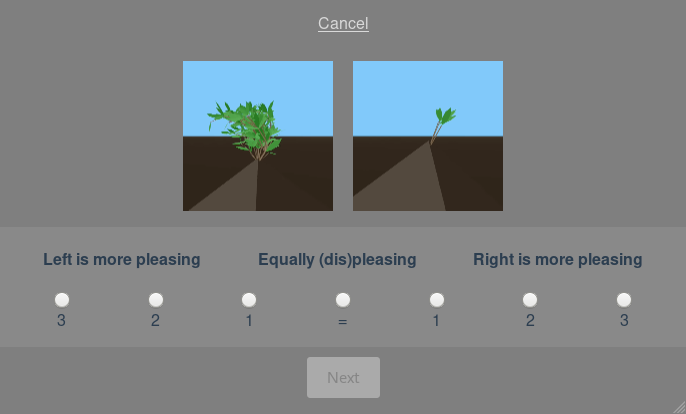
\includegraphics[width=1.0\textwidth]{figures/pairwise}
    \caption{Pairwise comparison task as viewed on a small screen}
    \label{fig:pairwise}
\end{figure}

Figure~\ref{fig:pairwise} shows the comparison task.
It is kept as simple as possible to avoid distractions, and a neutral gray background color is used to avoid the perceived hue or brightness of the plants to be shifted.
Two plants are visualized side by side as looping videos of a camera rotating around the plant such that all sides of the plant is seen.
In addition, the camera adjusts its height and distance from the plant so that all of the plant can be viewed.
The rotation happens at a balanced speed that lets the user view all of the plant in a short amount of time, while being slow enough to let them study it.
% The pilot confirmed that the speed was good.

The video runs at 60 frames per second (FPS) to give a smooth experience, to match the monitor refresh rate and to match what is commonly used in games.
They are encoded as both VP9 WebM and H.264 MPEG-4 to support a wide range of browsers.
According to Mozilla Developer Network (MDN), H.264 is supported in most browsers, but depends on platform support, and their support may be removed as the format has patents make them ``unfit for the open web platform''~\cite{mdn-video}.
Therefore the videos are encoded in both formats and VP9 is the preferred one if both are supported.

They are compressed as much as possible to reduce load times, while still keeping a near lossless visual quality as to not bias the comparisons.
Both are encoded with the FFmpeg tools\footnote{FFmpeg website: \url{http://ffmpeg.org/}}.
Both the FFmpeg Wiki and Google Developers recommend using Constant Quality for WebM~\cite{ffmpeg-vp9,google-vp9}.
They recommend CRF values from 15 to 35, and based on the resolution and Google Developers's resolution and CRF value matrix, a CRF of 32 is used~\cite{ffmpeg-vp9,google-vp9}.
For H.264, according FFMpeg Wiki a CRF value of 17--18 can be considered ``visually lossless''~\cite{ffmpeg-h264}.
Thus, 18 was selected as it allows the files to be smaller than 17.
Based on this, WebM is encoded with the parameters \texttt{-quality best -crf 32 -b:v 0}, while MPEG-4 is encoded with \texttt{-preset veryslow -crf 18}.
\texttt{-quality best} and \texttt{-preset veryslow} will enable better quality per file size at the cost of slower encoding~\cite{ffmpeg-h264}, but as the videos are encoded offline, the encoding time cost is not important.

The participant is presented with three categories to choose between: left is more pleasing, they are equally (dis)pleasing, and right is more pleasing.
If they find one more pleasing they need to rate how much pleasing it is on a scale of 1 to 3.
The original AHP method uses an 8-point scale,% cite
but this is too detailed for a ``normal human'',% cite or argue
and thus it was reduced to 3 points which allows for a low, medium and high rating.
Based on feedback from the pilot run, the ``equally (dis)pleasing'' option was labeled ``='' instead of ``0'' because ``0'' seemed like it meant that the plants were bad.
``(dis)'' was also added based on the feedback because without it it seemed like it meant that the plants were good.
With these changes, the participant should be less reluctant to select ``equal''.

By pressing the ``next'' button, the participant will be presented with new pairs until all have been rated.
The pairs are presented in random order and with random placement (left or right), as to not make the order create a bias.

\begin{figure}
    \centering
    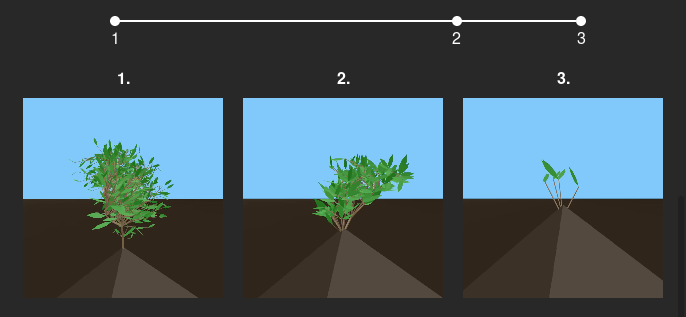
\includegraphics[width=1.0\textwidth]{figures/rank}
    \caption{Example rank resulting from human rating of plant pairs}
    \label{fig:rank}
\end{figure}

The post-questionnaire asks some questions and displays the resulting order of the plants.
Figure~\ref{fig:rank} shows an example of the resulting order.
The dots on the white line represents the relative distance between the plants, and the plants them selves are shown in order below.
% Explain how this is done.
In this example, the plant ranked as the best is much more better than the second than the second is to the third.
The participants are asked if they ``agree with the ranking of the plants shown below'', and if they do not ``strongly agree'', they are asked ``why do you not strongly agree with the ranking?''
This can help determine if the method of ranking the plants with AHP is valid.
Next they are asked the most important question: ``What would you say separates good plants from bad plants in the ranking?''
This is useful to be able to do a qualitative analysis of why the human ranking does not match the fitness ranking, if they do not match.
Finally, they are asked for ``other comments'' in case they have something useful to add that do not fit the other questions.

The final thank-you page contains a congratulation, a link to revisit their results, and a link to share the survey.
This share link contains a token that indicates who it was shared from.
With this data the snowball effect can be tracked.
Though, there is nothing preventing them from sharing the original link, thus losing this information.

\subsection{Implementation}
No web-based application the matches the design of the survey was found.
Thus as single-page web-application was created using the Vue.js JavaScript framework in the front end\footnote{Vue website: \url{https://vuejs.org/}}, the Rocket web framework for Rust in the back end\footnote{Rocket website: \url{https://rocket.rs/}}\footnote{Rust website: \url{https://www.rust-lang.org/}}, and MongoDB to store the data\footnote{MongoDB website: \url{https://www.mongodb.com/}}.
Multiple other libraries were used both in the front end and back end, but the aforementioned are the most central.
As the application is a on-off application, only meant to be used for the survey, and fairly simple, the choices of technology and architecture were based on experience, convenience and preferences.
Most of the technology used had recently been used in another project by the researcher, and thus allowed for code re-use and rapid development.

The application uses a client--server architecture, as shown in Figure~\ref{fig:pairwise-architecture}, where the server consists of two layers: API and DB.
The client uses a Vue Component for each page described in the Survey Design, and URL routing is handled by Vue Router.
The Components communicated directly to the API layer using a custom REST API, to for example register a participant or get the pairs of plants to evaluate.

The API layer is written in Rust and uses the Rocket framework to implement the API.
Multiple routes are defined based on the requirements of the client.
It communicates directly to the MongoDB database using the \textit{mongodb} Rust library.

When a participant registers, they receive a private token that is kept in the URL in the client throughout the whole survey.
This token access to submit and retrieve their data.
They also receive a public token that represents the participant, but does not grant access to their data.
Thus, this public token is used in the share link to identify who shared it.

The participant participates only in a specific \textit{task}.
A task is a set of plants that are to be evaluated, and the system may contain multiple tasks.
While only one task is used during the survey, allowing multiple tasks lets the researcher experiment with the application without affecting the real data while developing or during the survey.

The database contains three collections: \textit{user}, \textit{sample} and \textit{weight}.
\textit{user} stores all data relating to the user and is uniquely identified by the private and public tokens individually.
\textit{sample} stores data about one of the plants, such as its name and the task it is part of.
Finally, \textit{weight} stores the rating submitted by one user for one pair of plants and is uniquely identified by the user and the two plants together.

Finally there is a command-line interface (CLI) available to extract the data either as raw data or as calculated priority weights using AHP.
Because of this, a separate module \textit{stats} in the API layer contains the common functionality used by both the API and the CLI.

\subsection{Results}
\subsubsection{Participants}
There were 56 people that registered.
Of those, 37 completed ranking the plants.
This means that 34\% of the 56 participants did not rank the plant, of which many likely are people that unintentionally registered multiple times.
Those who did not complete the ranking of the plants will be excluded from the analysis.
Finally, one of the 37 did not submit the post questionnaire.

The demographic of the participants is mainly 20--30 year old (65\%) males (78\%) with a bachelor or higher degree (76\%) in information and communication technologies (49\%).
The age ranges from 21 to 69.
Science \& engineering and service \& sales were also strongly represented with 16\% and 14\% respectively.

There was only 1 participant that received the share link from another participant.
Still, only around 25 people were directly asked to participate, and only 15 confirmed that they participated.
Additionally, it is not expected that all of the people contacted directly did participate.
Thus, at least 12 participants, and likely more, must have received the link from another person.

% Analyze plant plant like/work and video game.

\subsubsection{Ranking Agreement}
\begin{figure}
    \centering
    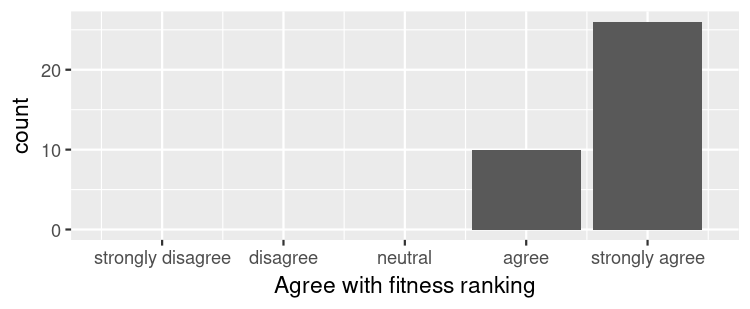
\includegraphics[width=0.7\textwidth]{figures/agree}
    \caption{Human agreement with the AHP ranking}
    \label{fig:agree}
\end{figure}

As seen in Figure~\ref{fig:agree}, the participants always agree with the ranking made by AHP.
73\% strongly agree, while the rest agree.
The ones that did not strongly agree have to explain why.
These explanations were categorized into four categories based on the content: null, invalid, position and distance, as shown in Table~\ref{tab:agree-why}.
While the participants were forced to write a reason, one participant was able to not write anything and is thus categorized as \textit{null}.
Some explanations contained comments that were not answering the question, which could be because of misunderstanding the question, misinterpretation of the scale, or laziness.
For example, the comment ``I never agree strongly with online tests'', indicates that they use the scale differently, and actually completely agree with the ranking.
Therefore, these comments were categorized as ``invalid''.
Finally, two categories were actual reasons to why they did not strongly agree: \textit{position} and \textit{distance}.
A plant being positioned in a wrong rank was the most common reason, as it was commented by 5 of the participants.
In all cases they only wanted to move one plant.
Only one commented on the distance between the ranks.

\begin{table}
    \centering
    \begin{tabularx}{\textwidth}{| l | X | l |}
    \hline
    \textbf{Category} & \textbf{Description} & \textbf{Occurrences} \\ \hline
    null & No comment & 1 \\
    \hline
    invalid & The participant did not answer the question, but commented something irrelevant & 3 \\
    \hline
    position & Feels that plant is in wrong position and wants to change its rank & 5 \\
    \hline
    distance & Feels that the distances between some ranks are either too short or too long & 1 \\
    \hline
    \end{tabularx}
    \caption{Reasons as to why 10 of the participants did not strongly agree with AHP ranking}
    \label{tab:agree-why}
\end{table}

\subsubsection{Correlation Between Human and Fitness Ranking}
\begin{figure}
    \centering
    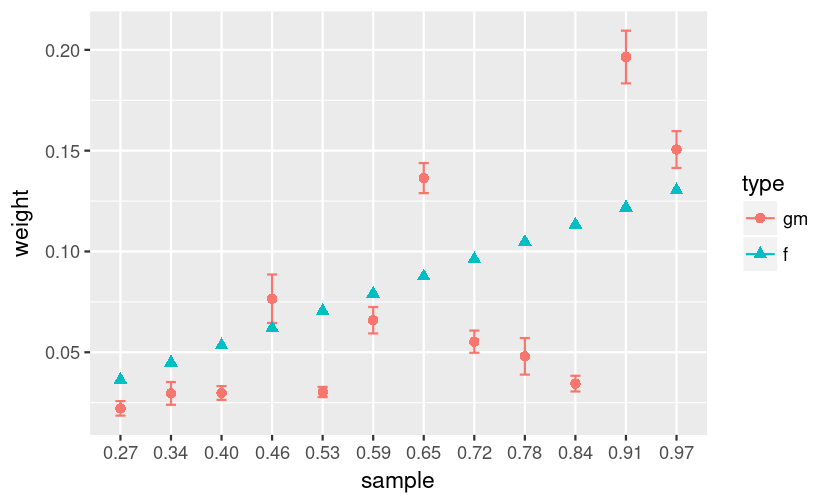
\includegraphics[width=1.0\textwidth]{figures/weights}
    \caption[Fitness score plus geometric mean and arithmetic mean of priority weights]{Normalized fitness score (f) plus geometric mean (gm) of human priority weights, with standard error}
    \label{fig:weights}
\end{figure}

The fitness ranking and the human aggregated ranking are shown together in Figure~\ref{fig:weights}.
From this it can be observed that both agree on the three worst and the two best rankings, while in-between these there are big differences.
For example, 0.65, 0.72, 0.78 and 0.84 are ordered in the reverse order, and are far from the fitness ranking.
0.53 and 0.84 is also ranked as bad as the three worst by the humans, while the fitness ranks them higher.
Finally, humans prefer 0.91 much more over 0.97, which is reverse of the fitness.
Still they do somewhat agree with the ranking of 0.49 and 0.59, while they are reversed.

dRank calculates a ranking distance of 16.67, and a p-value of 0, meaning that the human rankings are significantly different from the fitness ranking, and we reject the hypothesis that they are the same.
This does still not mean that there is no positive correlation between the rankings, only that they are not equal.
Kendall's tau is 0.55 (p < 0.05), indicating a positive correlation, though only at about 55\%.

With the two best ranks (0.97 and 0.91) and three worst ranks (0.27, 0.34, 0.40) removed, thus looking only at the ``middle'' part, the dRank distance is 5.21, still with a p-value of 0, and Kendall's tau is -0.33 (p >= 0.05), indicating no correlation in either direction (\textit{middle} in Table~\ref{tab:rankstats}).

% EXPLAIN HOW SCORES WERE TRANSLATED TO WEIGHTS FOR COMPARISON.

\subsubsection{Analysis of Bad Correlation}
\begin{figure}
    \centering
    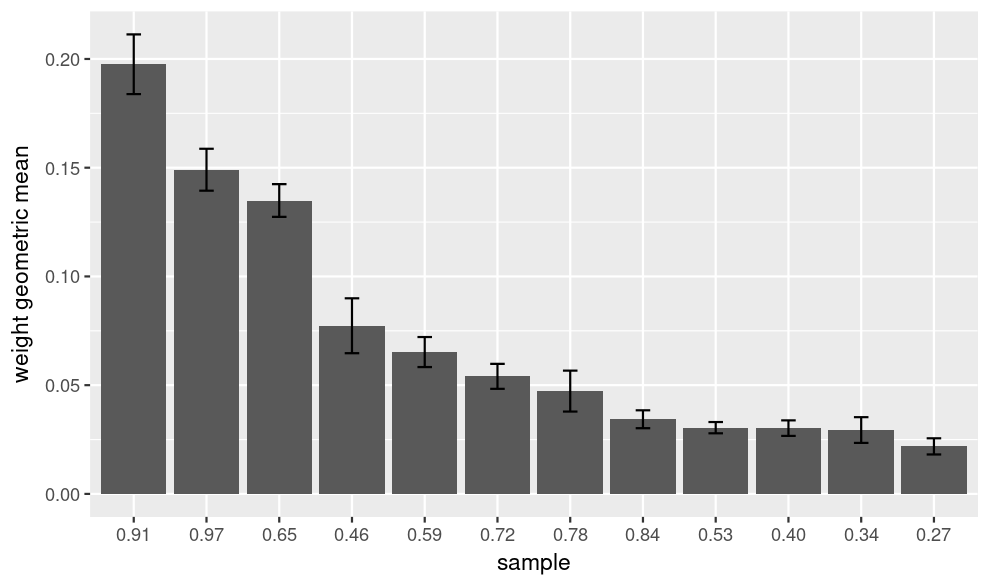
\includegraphics[width=1.0\textwidth]{figures/weights_bar}
    \caption[Priority weights from human plant ranking]{Priority weights from human plant ranking, with standard error}
    \label{fig:weights-bar}
\end{figure}

Figure~\ref{fig:weights-bar} shows the ordered human ranking.
Both agree that 0.27 is the worst plant.
0.34, 0.40, 0.53 and 0.84 seems to be ranked as equally bad, just above 0.27.
0.78, 0.72, 0.59 and 0.49 seem to be slightly climbing in score.
0.91 is clearly in first place, while 0.97 and 0.65 are possibly on a shared second place.
The standard errors are smaller on the bad plants than on the good plants.
Both 0.84 and 0.46 were moved 5 ranks down and up respectively, almost swapping places.
0.84 is the worst, having a difference in weight between its neighbor of 0.12 compared to 0.05 for the 0.46 plant.

\begin{figure}
    \centering
    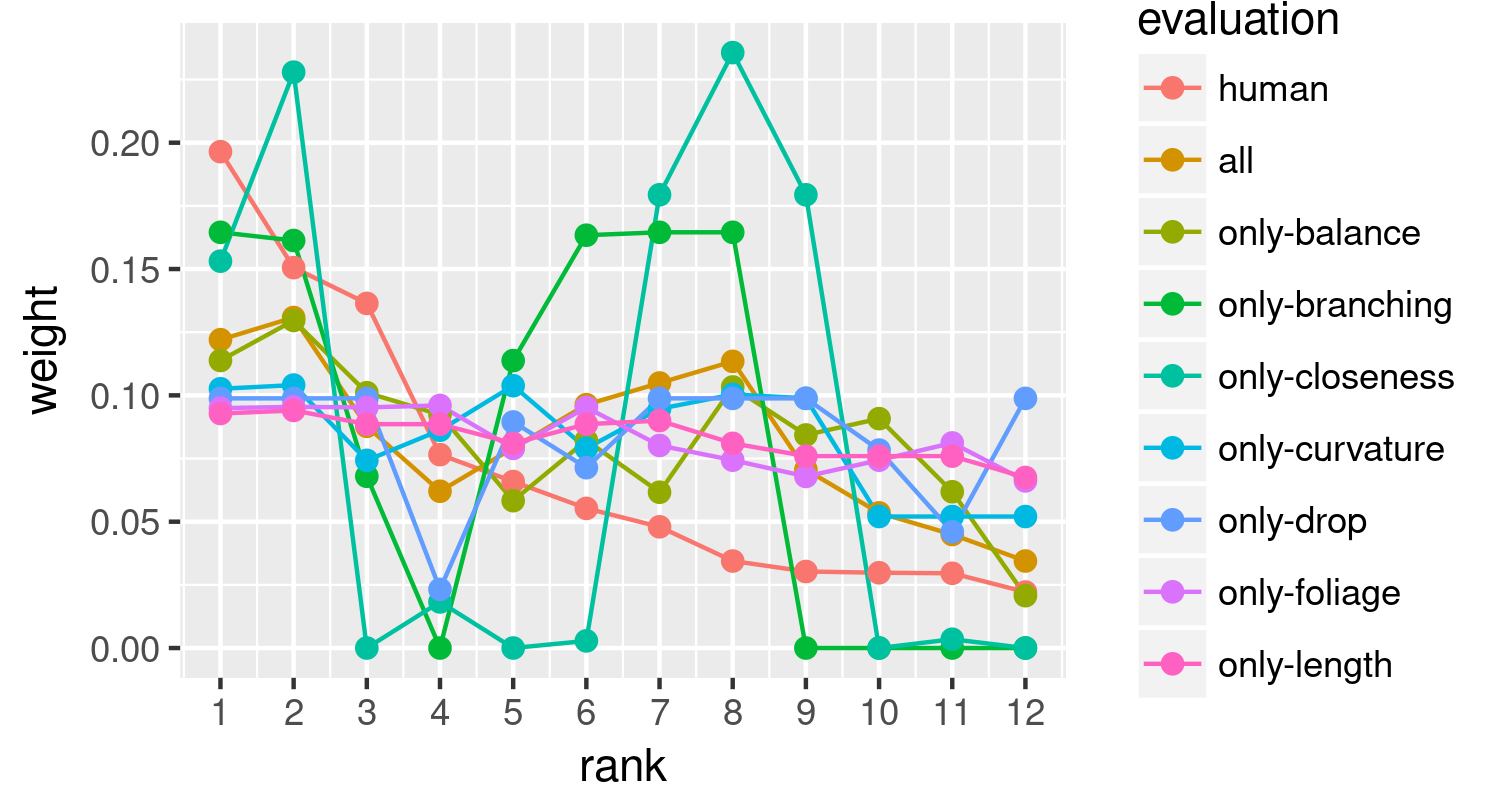
\includegraphics[width=1.0\textwidth]{figures/fitcmp-only}
    \caption[Human ranking compared to fitness ranking and its components]{Human ranking compared to fitness ranking (\textit{all}) and its components. The ranking on the x-axis is the human ranking.}
    \label{fig:fitcmp-only}
\end{figure}

\begin{table}
    \centering
    \begin{tabular}{| l | l | l |}
    \hline
    \textbf{Ranking} & \textbf{Kendall's Tau} & \textbf{dRank} \\
    \hline
                all & 0.55 (p = 0.01)  & 16.67 (p = 0) \\
             middle & -0.33 (p = 0.88) & 5.21 (p = 0) \\
        only-length & 0.75 (p = 0.00)  & 20.99 (p = 0) \\
       only-foliage & 0.57 (p = 0.01)  & 17.01 (p = 0) \\
       only-balance & 0.49 (p = 0.02)  & 16.67 (p = 0) \\
     only-curvature & 0.45 (p = 0.02)  & 16.63 (p = 0) \\
     only-branching & 0.36 (p = 0.07)  & 25.43 (p = 0) \\
     only-closeness & 0.14 (p = 0.27)  & 16.63 (p = 0) \\
          only-drop & 0.13 (p = 0.30)  & 21.67 (p = 0) \\
            removal & 0.79 (p = 0.00)  & 16.67 (p = 0) \\
     removal-middle & 0.52 (p = 0.07)  & 5.21 (p = 0) \\
    \hline
    \end{tabular}
    \caption{}
    \label{tab:rankstats}
\end{table}

% Should be in discussion?
Figure~\ref{fig:fitcmp-only} compares the human ranking against fitness ranking and each individual fitness metric.
The fitness ranking has a clear problem of scoring the ranks 5--9 too high, which creates a ``bump'' in the curve.
Two metrics that stand out --- closeness and branching --- look like may be a major cause of this bump, as they themselves have an even larger bump.
Additionally, the drop metric seems to be in a disagreement with the human ranking.
These observations are also supported by Kendall's Tau and to some degree dRank, as seen in Table~\ref{tab:rankstats}.
Kendall's Tau indicates that all three metrics are not correlated (p >= 0.05).
Branching also has a low correlation compared to the other metrics, but relatively higher than the other two.
dRank supports that drop and branching have a low correlation, but disagrees with Kendall's Tau on the closeness ranking.

\begin{figure}
    \centering
    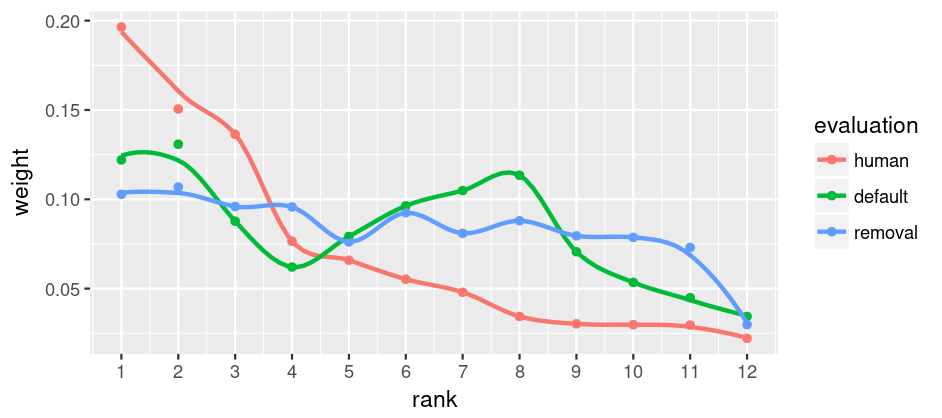
\includegraphics[width=1.0\textwidth]{figures/fitcmp-removal}
    \caption{}
    \label{fig:fitcmp-removal}
\end{figure}

These findings together suggest that these three metric may have a bad affect on the correlation of the human and fitness rankings.
This is supported by the plot of the \textit{removal} evaluation in Figure~\ref{fig:fitcmp-removal} and its rank correlation in Table~\ref{tab:rankstats} (\textit{removal}).
The ``bump'' has been removed, but there are instead some ``waves'' in the center part that disrupts the ranking.
Additionally, there is less distance between the two best plants and the third best plant, and a larger distance between the worst and second worst plants.
The Kendall's Tau is 0.79 (p < 0.05), which is an improvement of 0.24, while dRank indicates no difference.
Additionally, the correlation in the middle region has also improved as seen by \textit{removal-middle} in Table~\ref{tab:rankstats}, though Kendall's tau is still not statistically significantly different from 0 (p >= 0.05).

\subsubsection{Human Perception of Aesthetically Pleasing Plants}
All participants were asked openly what they would say ``separates good plants from bad plants in the ranking''.
These comments were categorized into factors and the number of participants who mentioned them was counted.
The factors were split into two: directional factors and directionless factors.
Directional factors have a clear understanding of what is better and what is worse, while directionless factors only understand what is important without knowing which direction is better or worse.
They can be found in Table~\ref{tab:factors-dir} and Table~\ref{tab:factors-nodir} respectively.

\begin{table}
    \centering
    \begin{tabularx}{\textwidth}{| l | X | l |}
    \hline
    \textbf{Category} & \textbf{Description} & \textbf{Occurrences} \\
    \hline
    natural & Looking ``natural'' is positive & 8 \\
    \hline
    artificial & Looking ``artificial'' is positive & 1 \\
    \hline
    healthy & Looking ``healthy'' is positive & 2 \\
    \hline
    details & Higher level of detail is positive & 4 \\
    \hline
    environment & Environmental effects on plants is positive & 3 \\
    \hline
    chaos & Chaos is negative & 5 \\
    \hline
    symmetry & Symmetry is positive & 1 \\
    \hline
    asymmetry & Symmetry is negative & 1 \\
    \hline
    patterns & Recognizable patterns is positive & 1 \\
    \hline
    more leaves & More leaves is positive & 5 \\
    \hline
    balanced leaves & Balanced amount of leaves is positive & 2 \\
    \hline
    lush & Higher leaf density is positive & 2 \\
    \hline
    leaf pitch & Leaves pointing up is positive & 1 \\
    \hline
    even spread & Branches and leaves spread out evenly is positive & 3 \\
    \hline
    small & Small plant size is negative & 3 \\
    \hline
    curves & More and soft curves is positive & 3 \\
    \hline
    upwards & Growing upwards is positive & 3 \\
    \hline
    sideways & Growing sideways is positive & 1 \\
    \hline
    complexity & Complex branches is positive & 2 \\
    \hline
    clipping & Branches or leaves growing inside the ground is negative & 2 \\
    \hline
    obstructions & Obstructions is positive & 1 \\
    \hline
    straight & When plants have few leaves they look better if they grow straight up & 1 \\
    \hline
    dynamic & Simple plants are better when dynamic & 1 \\
    \hline
    arrangement & Simple plants are better when well arranged & 1 \\
    \hline
    visible branches & Dense amounts of visible branches is negative & 1 \\
    \hline
    balanced & Center of mass close to trunk is positive & 1 \\
    \hline
    uniform bend & A uniform bend of the branches is positive & 1 \\
    \hline
    \end{tabularx}
    \caption{Directional factors}
    \label{tab:factors-dir}
\end{table}

\begin{table}
    \centering
    \begin{tabular}{| l | l |}
    \hline
    \textbf{Category} & \textbf{Occurrences} \\
    \hline
    leaf amount & 3 \\
    \hline
    leaf distribution & 2 \\
    \hline
    leaf density & 1 \\
    \hline
    leaf size & 1 \\
    \hline
    form & 3 \\
    \hline
    symmetry & 1 \\
    \hline
    growth & 1 \\
    \hline
    branch amount & 1 \\
    \hline
    branch placement & 1 \\
    \hline
    character & 1 \\
    \hline
    \end{tabular}
    \caption{Directionless factors}
    \label{tab:factors-nodir}
\end{table}

The abstract category ``natural'' was mentioned the most (8 times).
Many participants said that plants looking ``natural'' looked better, sometimes contrasted to ``artificial'' plants.
The word ``natural'' was often used as a dependent factor of other independent factors.
For example a comment said ``[...]the stems seemed to be perfect (angles), hence not natural'', which implies that ``natural'' is an important factor and the angles of the stems is a factor that affects the ``natural'' factor.
There was only one participant who suggested the opposite, i.e. that artificial-looking plants looked good, or more specifically ``interesting [...] as I do not expect to see a lot of symmetry in plants''.

``more leaves'' was the second most occurring category (5 comments).
Comments that fit into this category either suggest that the plants with more leaves look better, or that plants with less leaves look worse.
There were also comments that said that a balanced amount of leaves is positive (2 comments).

The third most occurring category is ``detail'', which says that a higher level of detail in the plants is a positive factor.
Simple or small plants were often commented as having too little detail and thus not looking natural.
There are three categories that are specifically for these types of plants: straight, dynamic and arrangement.
They suggest that simple plants look better when growing straight upwards, being more dynamic or well arranged.

\begin{table}
    \centering
    \begin{tabularx}{\textwidth}{| X | X | X | X |}
    \hline
    Abstract & Structure & Foliage & Other \\
    \hline
    natural, artificial, healthy, character, chaos, dynamic, growth, arrangement &
    symmetry, asymmetry, patterns, even spread, form, small, curves, upwards, sideways, complexity, visible branches, balanced, uniform bend, branch amount, straight, branch placement &
    more leaves, balanced leaves, lush, leaf pitch, leaf amount, leaf distribution, leaf density, leaf size &
    clipping, obstructions, details, environment \\
    \hline
    \end{tabularx}
    \caption{Grouping of factors}
    \label{tab:factor-groups}
\end{table}

The factors were grouped into four groups: abstract, structure, foliage and other.
The abstract group contains factors that are not quantifiable and thus more abstract in nature.
For example it is not straight forward to quantify how ``natural'' a plant looks.
Structure contains factors that consider the structure of the plant, i.e. the features of the branches and their patterns.
Foliage contains factors that consider the leaves on the plant and their individual properties or the foliage as a whole.
Other are factors that do not fit in the other groups.
The grouping of the factors is shown in Table~\ref{tab:factor-groups}.

% Turning off specific metrics mostly results in little change.
% Turning off branching improves the first valley and a little bit the bump, though it skews the bump to the right.
% Analyzing 0.53 and 0.84 indicates that the curvature may be rewarding plants that do not look curvy.
% Analyzing 0.46 it looks very lush, which may not be rewarded enough.
% Branching uses mean, but should use median.
% Curvature uses mean, but should use median.
% Length should be more cosine-like.
% Curvature should assume that the longest branch, not the ``straightest'', is the straight edge.
% Shorter segments and improved leaf heuristic could help with level of detail on small plants.
% Organic = natural

% "clean" interpreted as not chaotic.
% "foliage coverage" interpreted as "leaf distribution"
%
% Plant ranked 8 (0.84)
% - Looks artificial.
% - Few leaves
% - Not lush
% - Low level of detail?
% - Not growing upwards
% - Not complete
% - Center far from trunk
% - Metric says supurb curvature, but this is not visible
%
% Plant ranked 4 (0.46)
% - lush+
% - chaotic-
